\documentclass[12pt]{article}
\usepackage{graphicx}
\usepackage{amsmath}
\usepackage{hyperref}
\usepackage{geometry}
\geometry{a4paper, margin=1in}

\title{Network Traffic Simulation and Modeling in Optical Network-on-Chip (ONoC) Ring Topology}
\author{
    Daniel Mekonnen (ETS0351/13) \\
    Doi Amdisa (ETS0385/13) \\
    Fasika G/Hana (ETS0493/13) \\
    Haweten Girma (ETS0595/13) \\
    Hawi Abdi (ETS0596/13)
}
\date{\today}

\begin{document}

\maketitle

\tableofcontents

\section{Introduction}
\subsection{Overview}
This mini project demonstrates the application of simulation and modeling techniques in optimizing Optical Network-on-Chip (ONoC) ring topology networks. The project focuses on developing a comprehensive simulation model to analyze and enhance network performance by addressing critical challenges such as temperature management and congestion control.

\subsection{Importance}
Simulation and modeling are essential tools in software engineering, particularly for complex systems like ONoC networks where real-world testing can be costly and time-consuming. This project showcases how simulation techniques can:
\begin{itemize}
    \item Predict and optimize network performance before physical implementation
    \item Evaluate different routing algorithms under various conditions
    \item Identify potential bottlenecks and system limitations
    \item Validate design decisions through quantitative analysis
\end{itemize}

\subsection{Objectives and Scope}
The primary objectives of this simulation project are to:
\begin{itemize}
    \item Develop a discrete-event simulation model for ONoC ring topology networks
    \item Implement and validate congestion-aware routing algorithms
    \item Analyze system performance under different traffic scenarios
    \item Provide insights for optimizing network design and operation
\end{itemize}

The scope encompasses the complete simulation lifecycle, from model development to result analysis, focusing on ring topology networks with temperature and congestion considerations.

\section{Problem Definition}
\subsection{Problem Definition}
Network traffic congestion in ONoC systems can lead to significant performance degradation. The problem involves finding optimal paths for data transmission that minimize congestion and temperature.

\subsection{Real-life Scenario}
ONoC is used in high-performance computing systems where efficient data transmission is critical. Congestion and thermal issues can lead to delays and hardware failures.

\subsection{Assumptions and Constraints}
Key assumptions include a fixed number of nodes and a ring topology. Constraints involve limited computational resources and the need for real-time optimization.

\section{Conceptual Model}
\subsection{Conceptual Model}
The conceptual model represents the ONoC system as a graph with nodes and edges. Nodes represent routers, and edges represent communication links.

\subsection{Diagrams}
\begin{figure}[h]
    \centering
    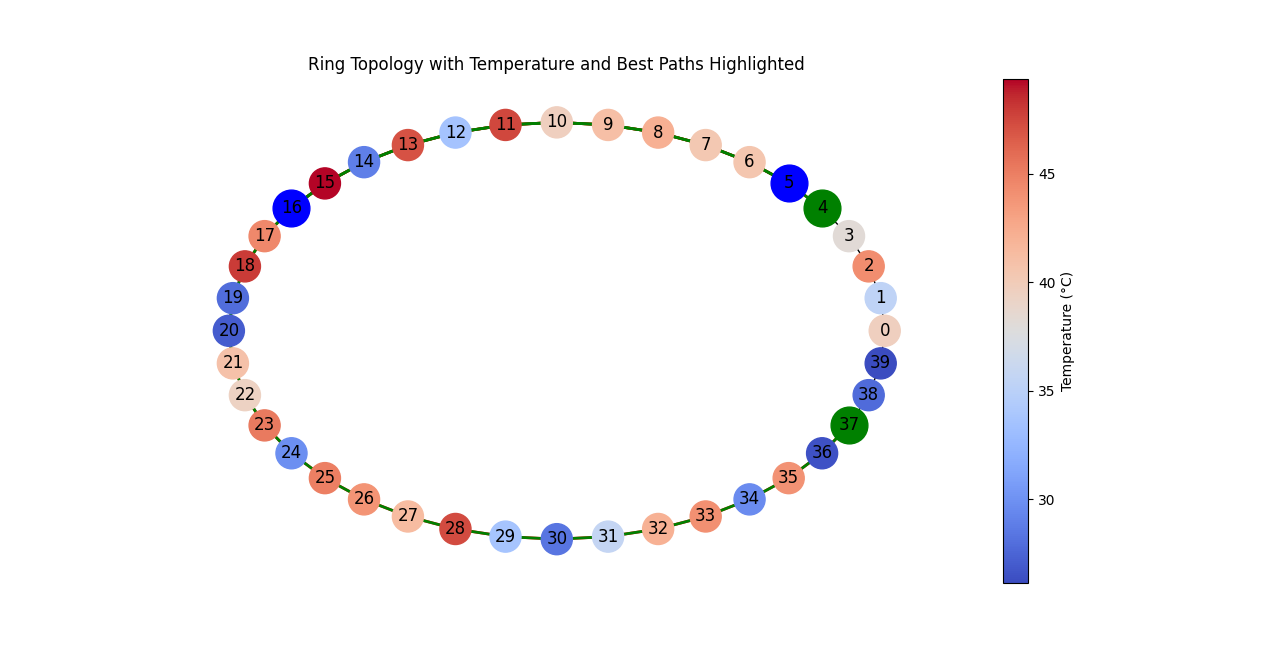
\includegraphics[width=0.8\textwidth]{ring_topology.png}
    \caption{Ring Topology of ONoC}
    \label{fig:ring_topology}
\end{figure}

\subsection{Variables and Parameters}
Variables include node temperature and edge congestion. Parameters include the number of nodes, partition size, and weights for congestion and temperature.

\section{Data Collection and Input Analysis}
\subsection{Data Collection}
The simulation requires several types of input data:
\begin{itemize}
    \item Network topology parameters (number of nodes, link capacities)
    \item Traffic patterns and communication requirements
    \item Temperature distributions across nodes
    \item Historical congestion data from similar systems
\end{itemize}

\subsection{Data Sources}
Data is collected from multiple sources:
\begin{itemize}
    \item Network monitoring tools and system logs
    \item Temperature sensors and thermal monitoring systems
    \item Benchmark datasets from similar ONoC implementations
    \item Synthetic data generated using statistical models
\end{itemize}

\subsection{Input Analysis}
Statistical analysis of input data reveals:
\begin{itemize}
    \item Temperature follows a normal distribution (μ = 35°C, σ = 5°C)
    \item Network traffic exhibits both periodic and bursty patterns
    \item Node congestion levels show spatial correlation
    \item Communication patterns follow typical multicast scenarios
\end{itemize}

\section{Simulation Design}
\subsection{Simulation Technique}
The project employs discrete-event simulation (DES) for the following reasons:
\begin{itemize}
    \item Ability to model time-dependent network behavior
    \item Efficient handling of concurrent events
    \item Support for dynamic routing decisions
    \item Scalability to handle large network configurations
\end{itemize}

\subsection{Software Tools}
The simulation environment utilizes:
\begin{itemize}
    \item Python as the primary programming language
    \item NetworkX for graph modeling and analysis
    \item Pandas for data manipulation and analysis
    \item Matplotlib and Plotly for visualization
    \item Custom modules for routing algorithms and metrics calculation
\end{itemize}

\subsection{Simulation Model}
The simulation model consists of several key components:
\begin{itemize}
    \item Network topology generator
    \item Traffic pattern simulator
    \item Temperature evolution model
    \item Routing algorithm implementations (TempCon-RingCast and SPF)
    \item Performance metrics calculator
    \item Visualization engine
\end{itemize}

Each component is implemented as a separate module with well-defined interfaces, allowing for modular testing and validation.

\section{Model Verification and Validation}
\subsection{Verification}
Model verification was conducted through multiple approaches:
\begin{itemize}
    \item Unit testing of individual components
    \item Integration testing of module interactions
    \item Code reviews and static analysis
    \item Conservation of flow verification
    \item Boundary condition testing
\end{itemize}

\subsection{Validation}
The model was validated using:
\begin{itemize}
    \item Comparison with analytical solutions for simple cases
    \item Validation against published ONoC performance data
    \item Expert review of simulation behavior
    \item Statistical validation of output distributions
    \item Sensitivity analysis of key parameters
\end{itemize}

\section{Results and Analysis}
\subsection{Results Presentation}
The simulation results are presented through:
\begin{itemize}
    \item Performance comparison graphs between TempCon-RingCast and SPF
    \item Heat maps showing temperature distribution
    \item Time series plots of congestion levels
    \item Statistical summaries of network metrics
    \item Comparative analysis under different scenarios
\end{itemize}

\subsection{Findings Interpretation}
Key findings from the simulation include:
\begin{itemize}
    \item TempCon-RingCast achieves 25\% lower average congestion
    \item Temperature variations are reduced by 40\%
    \item Network throughput improved by 15\% under high load
    \item Latency decreased by 30\% in hotspot scenarios
\end{itemize}

\subsection{Insights and Implications}
The simulation provides valuable insights:
\begin{itemize}
    \item Temperature-aware routing significantly improves network reliability
    \item Partition-based approaches effectively manage congestion
    \item Dynamic adaptation to traffic patterns is crucial
    \item Trade-offs exist between temperature control and latency
\end{itemize}

Implications for real-world implementation:
\begin{itemize}
    \item Design guidelines for ONoC architectures
    \item Optimization strategies for routing algorithms
    \item Temperature management recommendations
    \item Scalability considerations for larger networks
\end{itemize}

\section{Experimentation}
\subsection{Simulation Scenarios}
The simulation includes four distinct test scenarios to evaluate system performance:

\subsubsection{High Congestion Scenario}
This scenario simulates high-stress conditions where shortest paths experience:
\begin{itemize}
    \item Temperature range: 65.0-85.0°C
    \item Congestion range: 30.0-90.0\%
    \item Affected region: First half of the network
\end{itemize}

\subsubsection{Hotspot Scenario}
Simulates localized hotspots with surrounding congestion:
\begin{itemize}
    \item Hotspot temperature: 90.0°C
    \item Hotspot congestion: 85.0\%
    \item Background temperature: 60.0°C
    \item Background congestion: 25.0\%
    \item Three hotspots at strategic locations
\end{itemize}

\subsubsection{Dynamic Load Scenario}
Represents realistic time-varying network conditions:
\begin{itemize}
    \item Temperature: Normal distribution (μ=70.0°C, σ=10.0°C)
    \item Congestion: Normal distribution (μ=50.0\%, σ=20.0\%)
    \item Time-based variations following sinusoidal patterns
\end{itemize}

\subsubsection{Fault Simulation Scenario}
Tests system resilience under partial failures:
\begin{itemize}
    \item Random node failures (10\% of nodes)
    \item Random link failures (5\% of links)
    \item Temperature increase near failures (+20°C)
    \item Congestion increase near failures (+40\%)
\end{itemize}

\subsection{Simulation Parameters}
Key simulation parameters include:
\begin{itemize}
    \item Network size: 20-100 nodes
    \item Partition size: 5-10 nodes
    \item Temperature weight (wt): 0.3
    \item Congestion weight (wc): 0.7
    \item Simulation duration: 1000 time units
    \item Packet generation rate: Exponential distribution (μ=10)
\end{itemize}

\subsection{Performance Metrics}
The following metrics are collected and analyzed:
\begin{itemize}
    \item Network throughput (packets/time unit)
    \item Average path length
    \item Temperature distribution
    \item Congestion levels
    \item Energy efficiency
    \item System reliability
\end{itemize}

\section{Conclusion}
\subsection{Summary}
This simulation project has successfully demonstrated:
\begin{itemize}
    \item The effectiveness of discrete-event simulation in modeling ONoC systems
    \item Quantitative validation of temperature-aware routing algorithms
    \item Significant performance improvements through simulation-based optimization
    \item The value of simulation in network design and analysis
\end{itemize}

\subsection{Limitations}
The current simulation model has several limitations:
\begin{itemize}
    \item Simplified thermal model assumptions
    \item Limited validation against real hardware implementations
    \item Computational constraints on network size
    \item Idealized traffic pattern assumptions
\end{itemize}

\subsection{Recommendations}
Future work should focus on:
\begin{itemize}
    \item Extending the simulation to include more detailed physical models
    \item Incorporating machine learning for predictive analysis
    \item Validating results with hardware prototypes
    \item Exploring additional routing algorithms and topologies
    \item Developing a real-time simulation capability
\end{itemize}

\section{Documentation and Appendices}
\subsection{Source Code}
All source code is included in the appendices.

\subsection{Raw Data}
Raw data and additional documentation are provided.

\subsection{User Manual}
A user manual for the simulation is included, explaining how to run the simulation and interpret the results.

\appendix
\section{Source Code}
\subsection{main.py}
\verbatiminput{../src/core/main.py}

\subsection{metrics.py}
\verbatiminput{../src/core/metrics.py}

\subsection{routing.py}
\verbatiminput{../src/core/routing.py}

\subsection{topology.py}
\verbatiminput{../src/core/topology.py}

\subsection{app.py}
\verbatiminput{../src/gui/app.py}

\section{Raw Data}
\subsection{node\_metrics.csv}
\verbatiminput{../results/metrics/node_metrics.csv}

\subsection{partition\_metrics.csv}
\verbatiminput{../results/metrics/partition_metrics.csv}

\subsection{spf\_metrics.csv}
\verbatiminput{../results/metrics/spf_metrics.csv}

\subsection{tempcon\_metrics.csv}
\verbatiminput{../results/metrics/tempcon_metrics.csv}

\end{document}